\fancyhead{}
\fancyfoot{}
\cfoot{\thepage}

\lhead{Metodos}

\chapter{Metodos}

\section{Introducción }


Este capítulo describe el enfoque metodológico utilizado para desarrollar el Sistema Experto Basado en Reglas para el Monitoreo de Máquinas Críticas. Se detallan los métodos empleados en la recopilación de información, la formulación de reglas y la implementación del sistema. \\
\section{Enfoque}
En este estudio, se adoptó un enfoque cuantitativo basado en reglas para estructurar el conocimiento experto de la fábrica dentro del sistema. \\
Investigación Cuantitativa. \\
Se recopiló y analizó información técnica sobre el estado de las máquinas críticas, considerando parámetros medibles como temperaturas, caudal, y el estado de los compresores y bombas de agua. Esta información permitió definir umbrales de normalidad y anormalidad que fueron incorporados en el sistema experto. \\
\section{Diseño de la Investigación}
Dentro del enfoque cuantitativo, existen dos grandes clasificaciones de diseño de investigación: experimental y no experimental. Para este estudio, se ha adoptado un diseño no experimental, ya que no se manipulan variables de manera controlada, sino que se observan y analizan los estados de las máquinas en su entorno real de operación. \\
Diseño No Experimental \\
En este tipo de diseño, los datos se recopilan sin intervenir en los procesos naturales del sistema. Dentro de esta categoría, la investigación sigue un diseño longitudinal, pues se basa en la recolección continua de datos sobre el estado de las máquinas a lo largo del tiempo. \\

\section{Justificación del Diseño}
El Sistema Experto Basado en Reglas fue desarrollado para analizar información en tiempo real y detectar fallas en las máquinas críticas de la fábrica. Dado que las condiciones operativas varían constantemente, un diseño longitudinal permite evaluar tendencias, detectar anomalías y generar alarmas basadas en patrones históricos. \\
Este enfoque metodológico garantiza que el sistema pueda identificar problemas recurrentes, mejorar la toma de decisiones y mejorar las estrategias de mantenimiento sin necesidad de intervenir artificialmente en los procesos industriales. \\

\section{Fase de Diseño del Sistema Experto}
La fase de diseño fue clave para definir la estructura y los componentes fundamentales del sistema experto de monitoreo. Se llevaron a cabo distintas etapas para garantizar que el sistema fuera modular, eficiente y fácilmente escalable. \\
Diseño de la Arquitectura del Sistema Experto. \\
Se estableció la estructura general del sistema, identificando sus principales módulos y la forma en que interactúan entre sí. La arquitectura definida incluyó los siguientes componentes:

\section{Arquitectura del Sistema.} 

\begin{figure}[H]
    \begin{center}
    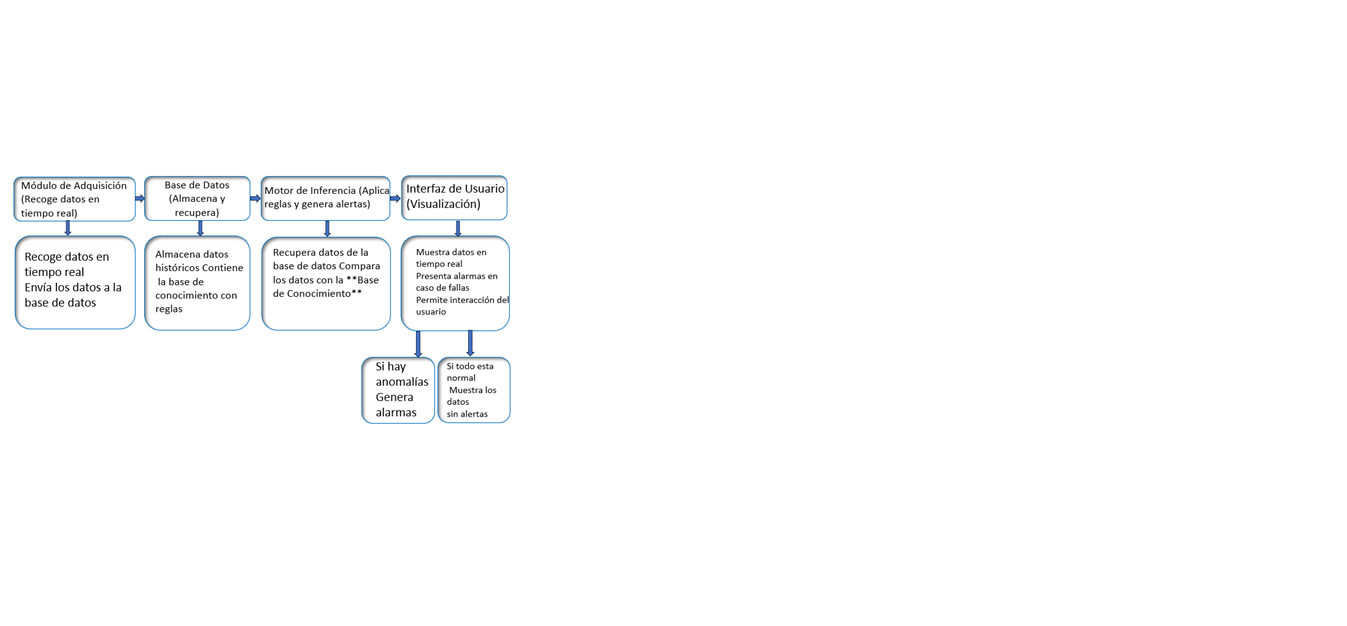
\includegraphics[scale = 1.0]{./images/Arquitectura del sistema experto.png}
    \caption{Arquitectura del sistema.}
    \label{fig:huella}
    \end{center}
    \end{figure}
Módulo de adquisición de datos: \\

Encargado de recibir información en tiempo real desde los sensores instalados en la fábrica. \\
\\
Base de conocimiento basada en reglas: \\
Contiene las reglas que permiten interpretar los datos y determinar el estado del sistema. \\
\\
Motor de inferencia: \\
Responsable de analizar los datos de entrada y aplicar las reglas para generar conclusiones y alertas. \\
\\

Interfaz de usuario:\\
Diseñada para permitir la visualización de datos en tiempo real y la interacción con el usuario. \\
\\
Base de datos:\\

Almacena los datos históricos del sistema y las reglas, asegurando un acceso eficiente. \\
Se definieron las interrelaciones entre estos módulos y el flujo de información que permite su correcto funcionamiento. \\
\\
Diseño de Módulos Funcionales. \\
Para garantizar un desarrollo eficiente y mantenible, el sistema se desglosó en módulos funcionales bien definidos: \\
Módulo de adquisición de datos: Responsable de la captura de datos de los sensores y su transmisión al sistema experto. \\

\begin{figure}[H]
    \begin{center}
    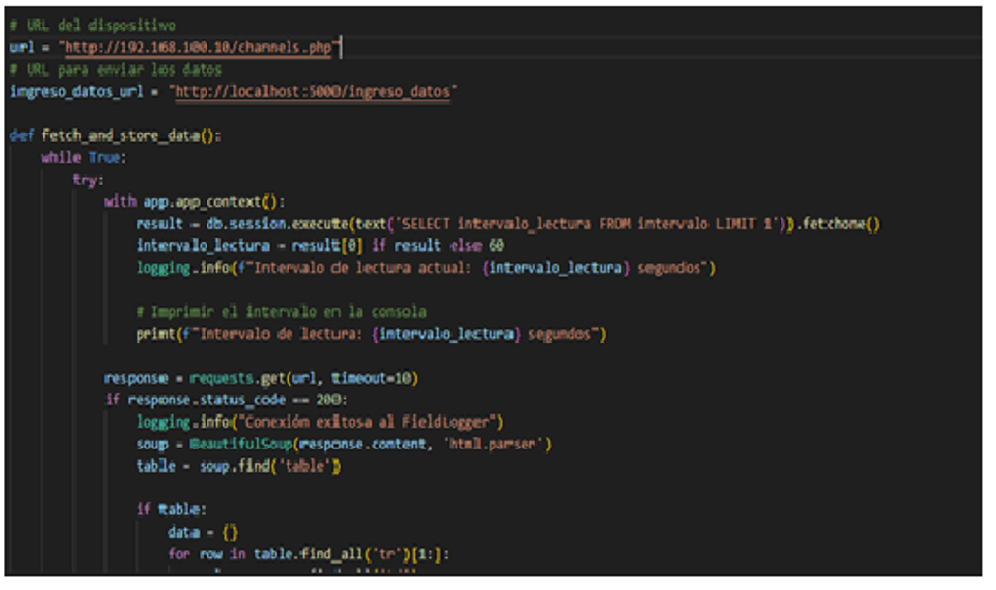
\includegraphics[scale = .5]{./images/Modulo de adquisicion de datos.png}
    \caption{Momdulo de adquisicion de datos.}
    \label{fig:huella}
    \end{center}
    \end{figure}

Módulo de procesamiento de datos: Normaliza y organiza la información para su análisis.\\
Módulo de inferencia: Implementa la lógica de decisión basada en reglas. \\
\\
Módulo de inferencia. \\

\begin{figure}[H]
    \begin{center}
    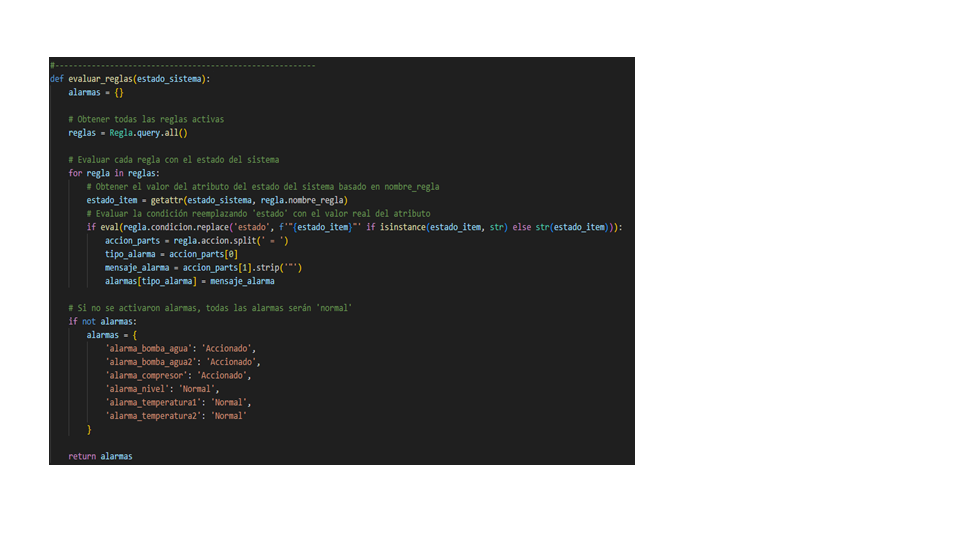
\includegraphics[scale = 0.7]{./images/motor de inferencia.png}
    \caption{Motor de inferencia.}
    \label{fig:huella}
    \end{center}
    \end{figure}


Módulo de visualización: Gestiona la interfaz web y la presentación de datos. \\
Cada módulo se diseñó con interfaces bien definidas para facilitar su integración y escalabilidad. \\

\begin{figure}[H]
    \begin{center}
    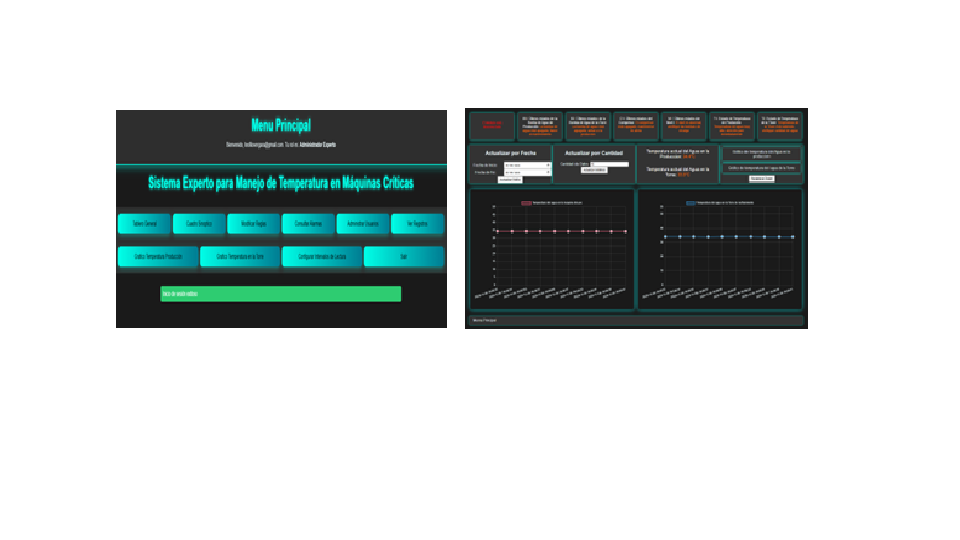
\includegraphics[scale = 0.6]{./images/desarrollo de sistema.png}
    \caption{Base de conocimiento.}
    \label{fig:huella}
    \end{center}
    \end{figure}


Diseño de la Base de Conocimiento \\
La base de conocimiento fue estructurada para facilitar su acceso y mantenimiento. Para ello, se determinaron los siguientes aspectos: \\

\begin{figure}[H]
    \begin{center}
    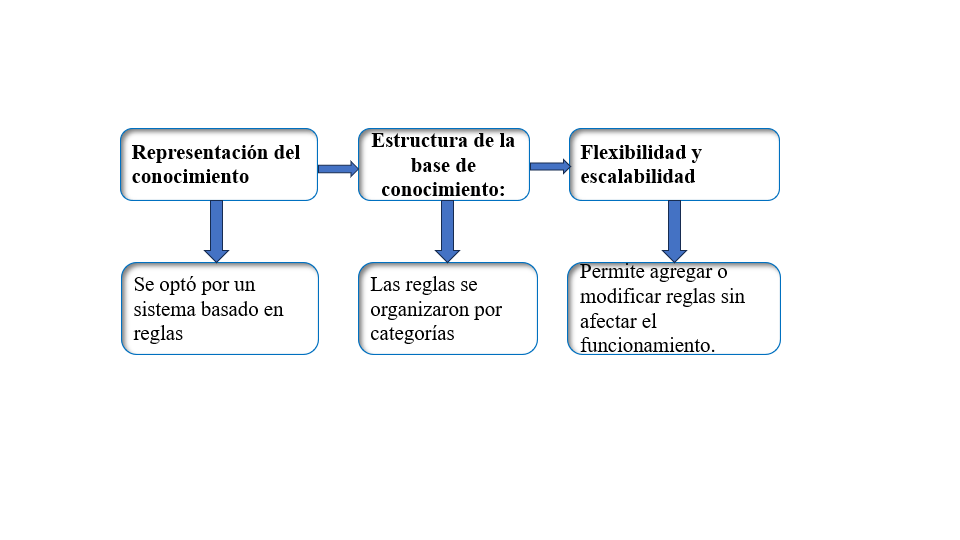
\includegraphics[scale = 0.6]{./images/base de conocimiento.png}
    \caption{Base de conocimiento.}
    \label{fig:huella}
    \end{center}
    \end{figure}

    \subsection{Representación del conocimiento: }
Se optó por un sistema basado en reglas, donde cada regla define un conjunto de condiciones y la acción a tomar en caso de que dichas condiciones se cumplan. \\
Estructura de la base de conocimiento: Las reglas se organizaron por categorías, agrupando aquellas relacionadas con parámetros específicos del sistema (bomba de agua, compresor, caudal, temperatura, etc.).\\
Flexibilidad y escalabilidad: Se diseñó un esquema que permite agregar o modificar reglas sin afectar el funcionamiento general del sistema. \\
\\
Diseño del Motor de Inferencia. 
El motor de inferencia es el encargado de procesar los datos adquiridos y aplicar las reglas de la base de conocimiento para tomar decisiones. \\
Selección del algoritmo de inferencia: Se utilizó un sistema basado en reglas condicionales para evaluar el estado del sistema en función de los datos obtenidos. \\
Optimización del rendimiento: Se definió una estrategia para minimizar el tiempo de respuesta y garantizar el análisis en tiempo real.
Integración con el módulo de adquisición de datos: Se estableció un mecanismo de comunicación eficiente para recibir datos en tiempo real y ejecutar las reglas de inferencia. \\
\\
Diseño de la Interfaz de Usuario\\
Se crearon prototipos de la interfaz web para asegurar una visualización clara y efectiva de la información generada por el sistema. \\
Visualización de datos en tiempo real: Se diseñaron gráficos dinámicos y paneles informativos para mostrar las mediciones del sistema. \\
\\
Gestión de alertas: Se implementó una sección donde el usuario puede ver las alertas generadas por el sistema y su causa. \\
\\

Experiencia de usuario: Se priorizó un diseño intuitivo y accesible, con una paleta de colores con fondo grafito y detalles en naranja oscuro. \\

Funcionamiento del Sistema Experto.\\
El sistema experto está diseñado para facilitar la gestión y monitoreo de los procesos industriales relacionados con los sistemas de refrigeración de agua en la producción de PVC. El sistema está estructurado en base a un esquema de usuarios con diferentes roles, lo que permite una administración eficiente de las funcionalidades según el perfil de cada usuario. \\
Inicio de Sesión (Login) y Roles de Usuario. \\
Al ingresar al sistema, el usuario debe autenticar sus credenciales a través del login. El sistema permite acceder a diferentes secciones dependiendo del rol asignado al usuario. Los roles definidos incluyen: \\
Administrador.\\
Los usuarios con privilegios de Administrador pueden acceder a una sección especial que les permite agregar, editar o eliminar usuarios. Además, pueden asignar o modificar roles a los usuarios, asegurando que las funciones y permisos estén correctamente distribuidos en la organización. Esta funcionalidad garantiza que solo los usuarios adecuados tengan acceso a áreas sensibles del sistema. \\
\\
Administrador experto. \\
Los Administradores expertos tienen la capacidad de modificar las reglas del sistema experto a través de una interfaz dedicada. Estas reglas están relacionadas con el monitoreo de los sistemas críticos de refrigeración. Por ejemplo, un administrador de reglas puede modificar umbrales de temperatura o establecer condiciones de alarma. Esta flexibilidad asegura que el sistema se adapte a diferentes condiciones operativas. \\
Operador: \\
Accede principalmente a las funcionalidades de consulta y visualización, pero con permisos limitados. \\
Cada usuario se verá redirigido a una página principal donde podrá ver las opciones disponibles basadas en su rol. El sistema garantiza que cada usuario solo tenga acceso a las funciones que le corresponden según su perfil. \\
Visualización de Temperaturas.\\
Una de las funcionalidades clave del sistema es la visualización gráfica de las temperaturas de los sistemas de refrigeración. En una página dedicada, se muestra una gráfica en tiempo real con los datos de temperatura recogidos desde el sistema. Los usuarios pueden observar el comportamiento de las temperaturas y detectar posibles desviaciones en el funcionamiento de la maquinaria. Esta página es crucial para los técnicos, ya que les permite identificar rápidamente cualquier irregularidad que pueda afectar el rendimiento del sistema de refrigeración.\\
\\
Cuadro Sinóptico. \\

Otra página importante es el cuadro sinóptico, que proporciona una vista global del estado de todos los sistemas de refrigeración. Esta página se actualiza dinámicamente a partir de los datos almacenados en la base de datos. Los usuarios pueden consultar en tiempo real el estado de cada equipo, incluidas las alarmas activas y las condiciones operativas de los sistemas de refrigeración. Esto permite un monitoreo constante y oportuno, facilitando la detección de fallos y la implementación de acciones correctivas inmediatas.\\

\begin{figure}[H]
\begin{center}
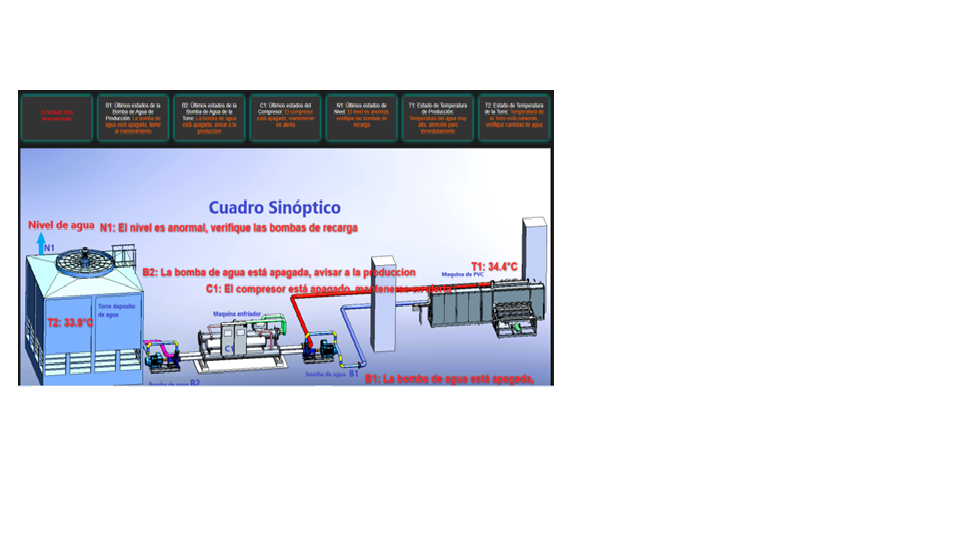
\includegraphics[scale = 0.9]{./images/cuadro sinoptico.png}
\caption{Cuadro sinóptico.}
\label{fig:huella}
\end{center}
\end{figure}

\subsection{Partes principales del código fuente}

\begin{figure}[H]
\begin{center}
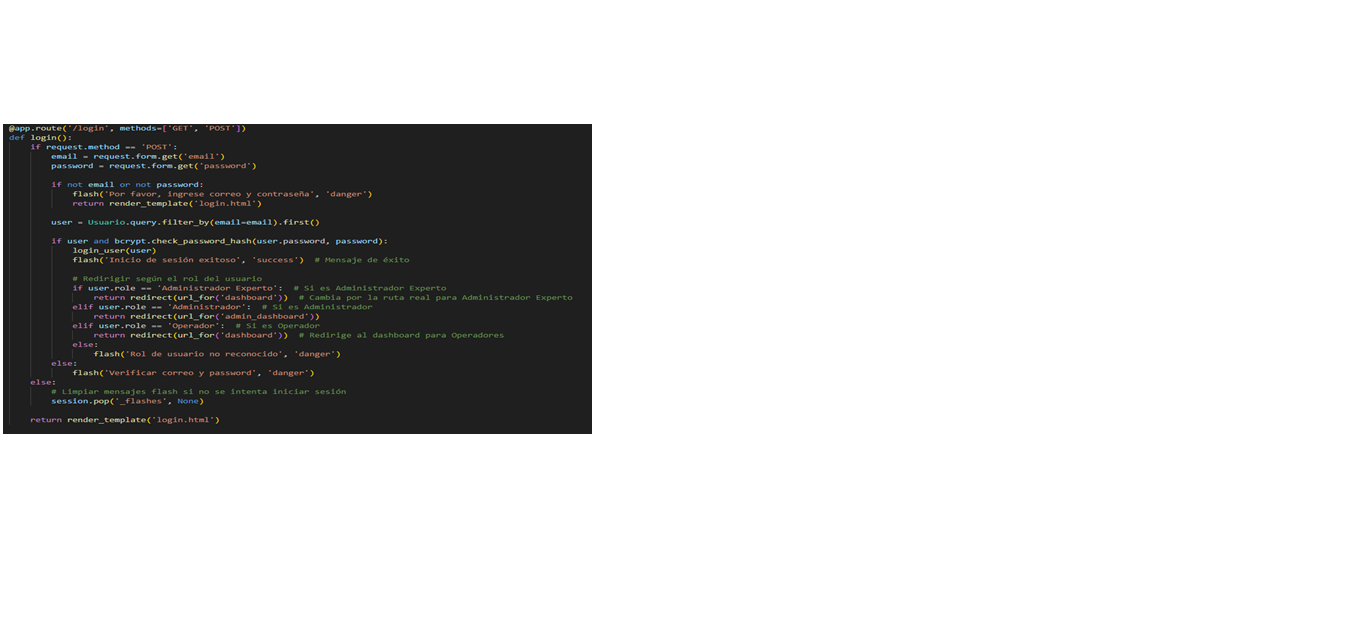
\includegraphics[scale = 0.8]{./images/codigo de login.png}
\caption{Codigo de login.}
\label{fig:huella}
\end{center}
\end{figure}

\begin{figure}[H]
\begin{center}
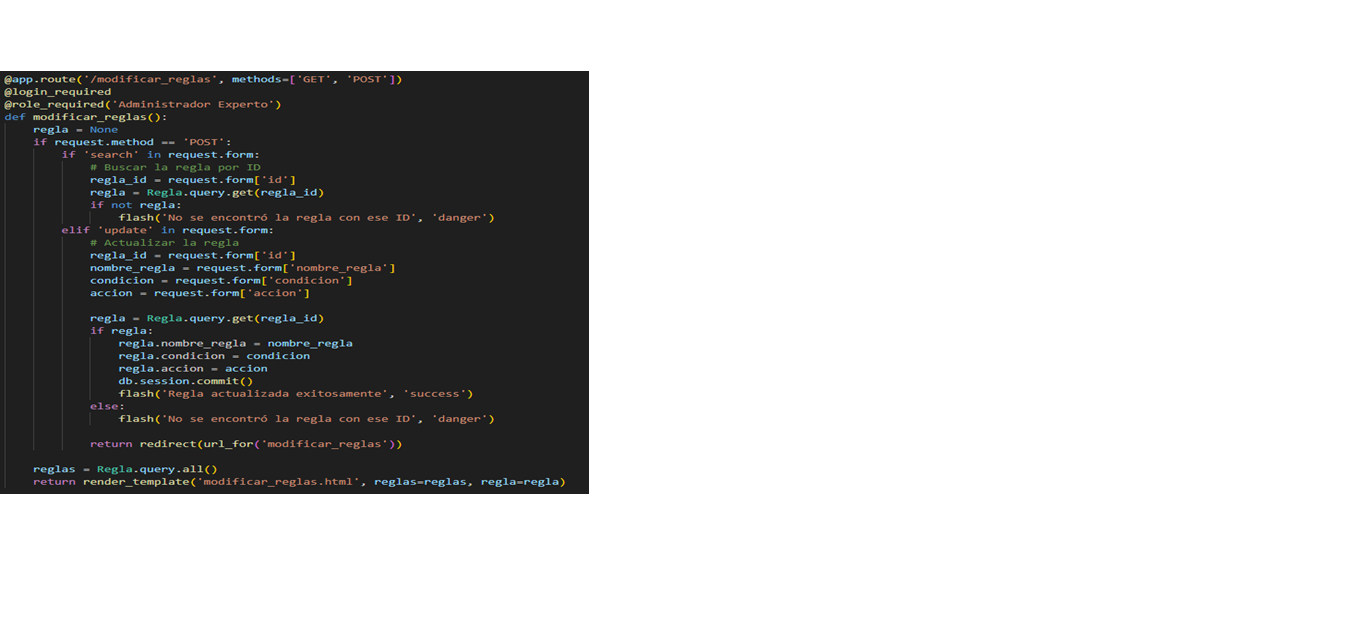
\includegraphics[scale = 0.8]{./images/modificar reglas.png}
 \caption{Codigo para modificar reglas.}
\label{fig:huella}
\end{center}
\end{figure}

\begin{figure}[H]
    \begin{center}
     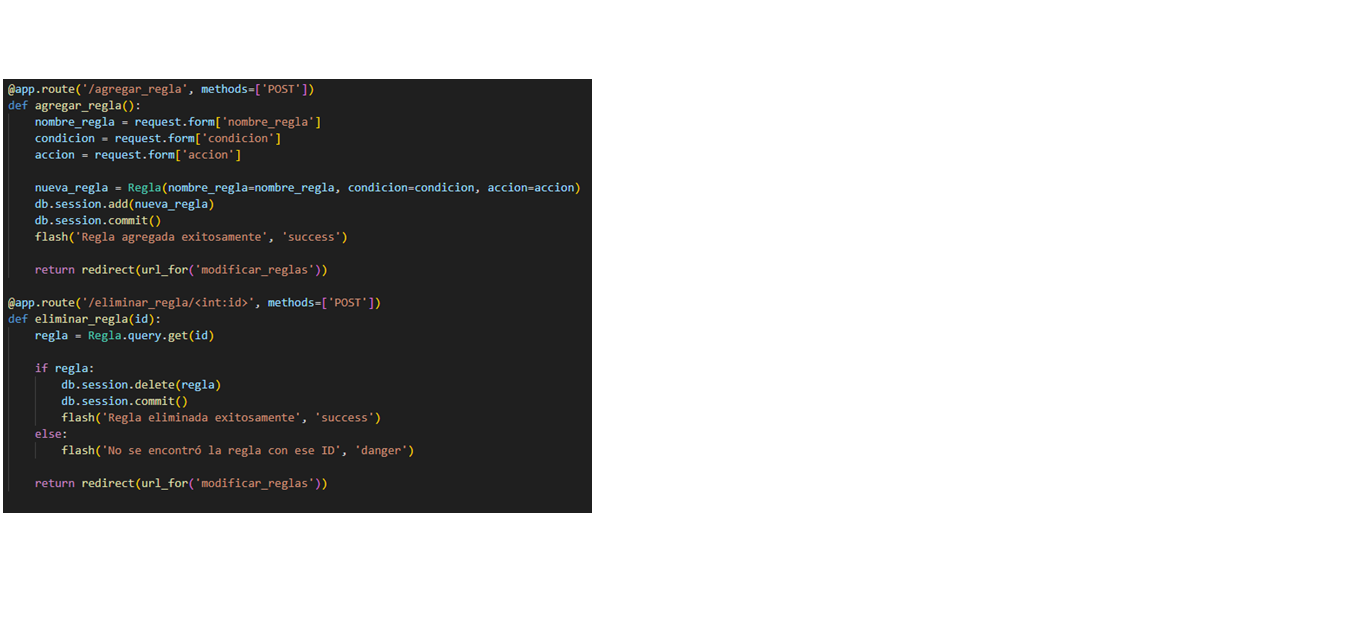
\includegraphics[scale = 0.8]{./images/agregar eliminar.png}
     \caption{Agregar o modificar reglas.}
     \label{fig:huella}
    \end{center}
    \end{figure}

            \begin{figure}[H]
                \begin{center}
                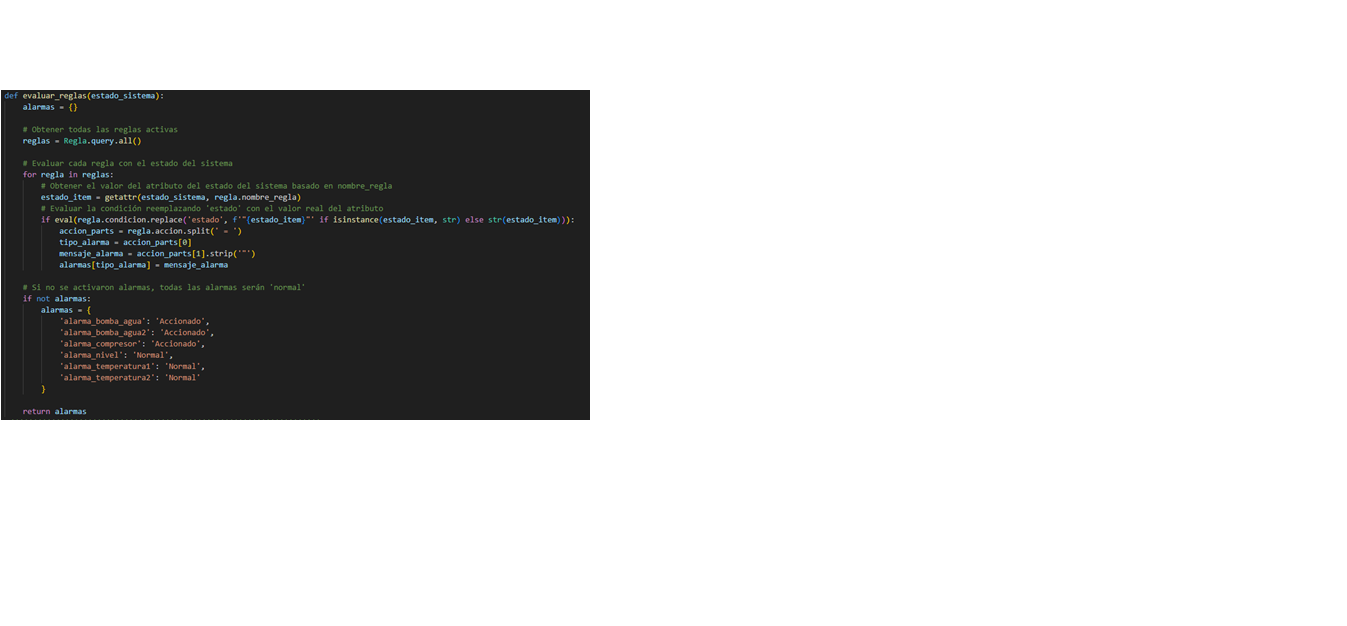
\includegraphics[scale = 0.8]{./images/evaluar reglas.png}
                \caption{Evaluar reglas.}
                \label{fig:huella}
                \end{center}
                \end{figure}
    
